\documentclass[14pt,a4paper,oneside]{extbook}
\usepackage[utf8]{vietnam}
\usepackage{amsmath,amssymb,mathrsfs,fancyhdr,enumerate,multirow,makecell}
\usepackage{tkz-euclide,tikz-3dplot,tikz,tkz-tab}
\usetikzlibrary{arrows.meta,calc,intersections,angles,quotes,backgrounds,shapes.geometric,patterns,through,shadows,positioning}
\usepackage{yhmath}
\usepackage[top=0.7cm, bottom=0.7cm, left=1.0cm, right=1.0cm, headheight=16pt, headsep=3mm, footskip=5mm]{geometry}
\usepackage[hidelinks,unicode]{hyperref}
\usepackage{qrcode}
\usepackage[many]{tcolorbox}
\usepackage{fontawesome}

\pagestyle{fancy}
\fancyhf{}
\fancyhead[L]{\footnotesize\bfseries\color{teal!85!black}\faBook~SỔ TAY KIẾN THỨC TOÁN 4}
\fancyhead[R]{\footnotesize\bfseries\color{blue!85!black}Lớp Toán Thầy Lĩnh -- loptoanthaylinh.vn}
\fancyfoot[C]{\footnotesize\bfseries\color{gray!80!black}-- Sổ tay kiến thức: Bài 18. Đề-xi-mét vuông, mét vuông, mi-li-mét vuông --}
\renewcommand{\headrulewidth}{0.4pt}

\begin{document}

% --- BANNER TIÊU ĐỀ BÀI HỌC ---
\noindent
\begin{tcolorbox}[
  enhanced,
  colback=teal!8!white,
  colframe=teal!80!black,
  arc=3mm, boxrule=1pt,
  left=3mm, right=3mm, top=2mm, bottom=2mm,
  halign=center
]
  {\Large\bfseries\color{teal!90!black}\faBookmark\ BÀI 18: ĐỀ-XI-MÉT VUÔNG, MÉT VUÔNG, MI-LI-MÉT VUÔNG}\\[1.5pt]
  {\footnotesize\itshape\color{black!75} Khái niệm diện tích vuông, mối liên hệ hệ số 100 và kĩ năng đổi đơn vị diện tích trên 1 trang A4}
\end{tcolorbox}

\vspace{2mm}

% --- KHỐI 1 & 2: LÝ THUYẾT & KĨ NĂNG ---
\noindent
\begin{minipage}[t]{0.49\textwidth}
  \begin{tcolorbox}[
    enhanced,
    title={\footnotesize\bfseries\color{white}\faThLarge\ 1. Khái niệm đơn vị diện tích},
    colback=blue!2!white,
    colframe=blue!75!black,
    arc=2.5mm, boxrule=0.8pt, top=1.8mm, bottom=1.8mm, left=2mm, right=2mm
  ]
    \footnotesize
    $\bullet$ \textbf{Mét vuông ($\text{m}^2$)}: Diện tích hình vuông có cạnh dài $1\text{ m}$.\\
    $\bullet$ \textbf{Đề-xi-mét vuông ($\text{dm}^2$)}: Diện tích hình vuông có cạnh dài $1\text{ dm}$.\\
    $\bullet$ \textbf{Mi-li-mét vuông ($\text{mm}^2$)}: Diện tích hình vuông có cạnh dài $1\text{ mm}$.\\
    $\bullet$ \textbf{Bảng đơn vị diện tích theo thứ tự}:
    \begin{center}
      $\mathbf{m^2} \quad \rightarrow \quad \mathbf{dm^2} \quad \rightarrow \quad \mathbf{cm^2} \quad \rightarrow \quad \mathbf{mm^2}$
    \end{center}
    Mỗi đơn vị đo diện tích gấp \textbf{100 lần} đơn vị bé hơn liền sau nó.
  \end{tcolorbox}
\end{minipage}%
\hfill
\begin{minipage}[t]{0.49\textwidth}
  \begin{tcolorbox}[
    enhanced,
    title={\footnotesize\bfseries\color{white}\faExchange\ 2. Mối quan hệ giữa các đơn vị},
    colback=teal!2!white,
    colframe=teal!75!black,
    arc=2.5mm, boxrule=0.8pt, top=1.8mm, bottom=1.8mm, left=2mm, right=2mm
  ]
    \footnotesize
    $\bullet$ \textbf{Hệ số chuyển đổi liền kề}: $\times 100$ hoặc $: 100$.\\
    --- $1\text{ m}^2 = 100\text{ dm}^2$\\
    --- $1\text{ dm}^2 = 100\text{ cm}^2$\\
    --- $1\text{ cm}^2 = 100\text{ mm}^2$\\[1mm]
    $\bullet$ \textbf{Chuyển đổi nhảy bậc}:\\
    --- $1\text{ m}^2 = 10\,000\text{ cm}^2 = 1\,000\,000\text{ mm}^2$\\
    --- $1\text{ dm}^2 = 10\,000\text{ mm}^2$\\
    $\bullet$ \textbf{Quy tắc viết}: Mỗi đơn vị diện tích tương ứng với đúng \textbf{2 chữ số}.
  \end{tcolorbox}
\end{minipage}

\vspace{2mm}

% --- KHỐI 3: SƠ ĐỒ TƯ DUY TIKZ ---
\noindent
\begin{tcolorbox}[
  enhanced,
  title={\footnotesize\bfseries\color{white}\faSitemap\ SƠ ĐỒ TƯ DUY: BẬC THANG QUY ĐỔI ĐƠN VỊ DIỆN TÍCH ($\times 100$)},
  colback=yellow!2!white,
  colframe=orange!85!black,
  arc=2.5mm, boxrule=0.8pt, top=1.5mm, bottom=1.5mm, left=1mm, right=1mm,
  halign=center
]
  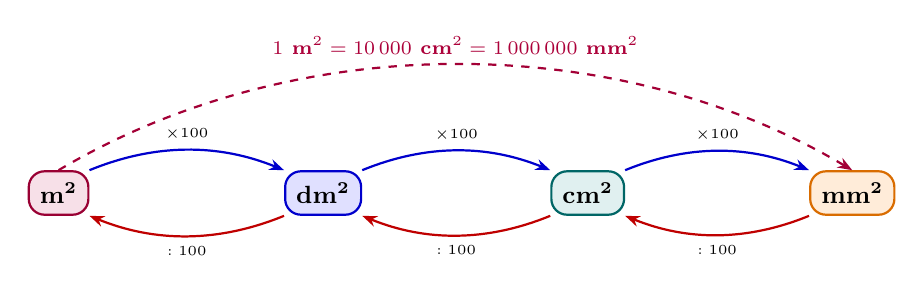
\begin{tikzpicture}[
    xscale=1.2, yscale=0.85,
    unit/.style={rectangle, rounded corners=2mm, draw=teal!80!black, fill=teal!12, thick, inner sep=4pt, font=\small\bfseries, align=center},
    arr_top/.style={-{Stealth[scale=0.8]}, thick, draw=blue!80!black},
    arr_bot/.style={-{Stealth[scale=0.8]}, thick, draw=red!75!black}
  ]
    \node[unit, fill=purple!12, draw=purple!80!black] (m2) at (0,0) {$\mathbf{m^2}$};
    \node[unit, fill=blue!12, draw=blue!80!black] (dm2) at (2.8,0) {$\mathbf{dm^2}$};
    \node[unit, fill=teal!12, draw=teal!80!black] (cm2) at (5.6,0) {$\mathbf{cm^2}$};
    \node[unit, fill=orange!15, draw=orange!85!black] (mm2) at (8.4,0) {$\mathbf{mm^2}$};

    % Mũi tên trên x100 (2 số 0)
    \draw[arr_top] (m2.north east) to[bend left=30] node[above, font=\tiny\bfseries]{$\times 100$} (dm2.north west);
    \draw[arr_top] (dm2.north east) to[bend left=30] node[above, font=\tiny\bfseries]{$\times 100$} (cm2.north west);
    \draw[arr_top] (cm2.north east) to[bend left=30] node[above, font=\tiny\bfseries]{$\times 100$} (mm2.north west);

    % Mũi tên nhảy bậc
    \draw[arr_top, dashed, draw=purple!85!black] (m2.north) to[bend left=40] node[above, font=\scriptsize\bfseries\color{purple!90!black}]{$1\text{ m}^2 = 10\,000\text{ cm}^2 = 1\,000\,000\text{ mm}^2$} (mm2.north);

    % Mũi tên dưới :100
    \draw[arr_bot] (mm2.south west) to[bend left=30] node[below, font=\tiny\bfseries]{$: 100$} (cm2.south east);
    \draw[arr_bot] (cm2.south west) to[bend left=30] node[below, font=\tiny\bfseries]{$: 100$} (dm2.south east);
    \draw[arr_bot] (dm2.south west) to[bend left=30] node[below, font=\tiny\bfseries]{$: 100$} (m2.south east);
  \end{tikzpicture}
\end{tcolorbox}

\vspace{2mm}

% --- KHỐI 4: VÍ DỤ MINH HỌA & BẪY TRẮC NGHIỆM ---
\noindent
\begin{minipage}[t]{0.53\textwidth}
  \begin{tcolorbox}[
    enhanced,
    title={\footnotesize\bfseries\color{white}\faCheckCircle\ Ví dụ thực hành chuẩn mực},
    colback=green!2!white,
    colframe=green!60!black,
    arc=2.5mm, boxrule=0.8pt, top=1.8mm, bottom=1.8mm, left=2.2mm, right=2.2mm
  ]
    \footnotesize
    $\bullet$ \textbf{Ví dụ 1 (Đổi xuôi):}\\
    $5\text{ m}^2\ 30\text{ dm}^2 = 500\text{ dm}^2 + 30\text{ dm}^2 = \mathbf{530\text{ dm}^2}$.\\
    $2\text{ dm}^2\ 8\text{ cm}^2 = 200\text{ cm}^2 + 8\text{ cm}^2 = \mathbf{208\text{ cm}^2}$.\\
    $\bullet$ \textbf{Ví dụ 2 (Đổi ngược):}\\
    $450\text{ cm}^2 = 400\text{ cm}^2 + 50\text{ cm}^2 = \mathbf{4\text{ dm}^2\ 50\text{ cm}^2}$.\\
    $3\,000\,000\text{ mm}^2 = \mathbf{3\text{ m}^2}$.
  \end{tcolorbox}
\end{minipage}%
\hfill
\begin{minipage}[t]{0.45\textwidth}
  \begin{tcolorbox}[
    enhanced,
    title={\footnotesize\bfseries\color{white}\faExclamationTriangle\ Mẹo tránh bẫy trắc nghiệm},
    colback=red!2!white,
    colframe=red!70!black,
    arc=2.5mm, boxrule=0.8pt, top=1.8mm, bottom=1.8mm, left=2.2mm, right=2.2mm
  ]
    \footnotesize
    $\bullet$ \textbf{Bẫy hệ số 10 của độ dài:}\\
    Nhiều học sinh quen $1\text{ m} = 10\text{ dm}$ nên viết $1\text{ m}^2 = 10\text{ dm}^2$ $\rightarrow$ \textbf{RẤT SAI}! Phải là \textbf{100}.\\
    $\bullet$ \textbf{Bẫy khuyết chữ số 0:}\\
    $2\text{ dm}^2\ 5\text{ cm}^2 \ne 25\text{ cm}^2$ mà phải là $\mathbf{205\text{ cm}^2}$ (vì mỗi đơn vị có 2 chữ số: 05).
  \end{tcolorbox}
\end{minipage}

\end{document}
